% -------------------------------
\mysec{Satzgruppe des Pythagoras}
% -------------------------------
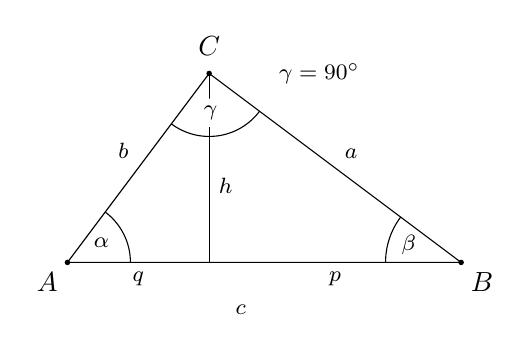
\begin{tikzpicture}[scale=0.2]
  % Linien
  \draw ( 0,  0) -- node[below]       {{\footnotesize$q$}}
        ( 9,  0) -- node[below]       {{\footnotesize$p$}}
        (25,  0) -- node[above right] {{\footnotesize$a$}}
        ( 9, 12) -- node[above left]  {{\footnotesize$b$}}
        ( 0,  0);
  \draw ( 9,  0) -- node[below right] {{\footnotesize$h$}}
        ( 9, 12);
  \node at (11, -3)                   {{\footnotesize$c$}};
  % Punkte
  \fill ( 0,  0) circle (5pt) node[below left]  {$A$};
  \fill (25,  0) circle (5pt) node[below right] {$B$};
  \fill ( 9, 12) circle (5pt) node[above=1mm]   {$C$};
  % alpha
  \begin{scope}
    \clip (0, 0) -- (25, 0) -- (9, 12) -- cycle;
    \draw (0, 0) circle (4);
    \node[shift=(30:5mm)] at (0, 0) {{\footnotesize$\alpha$}};
  \end{scope}
  % beta
  \begin{scope}
    \clip (0, 0) -- (25, 0) -- (9, 12) -- cycle;
    \draw (25, 0) circle (4.8);
    \node[shift=(162:7mm)] at (25, 0) {{\footnotesize$\beta$}};
  \end{scope}
  % gamma
  \begin{scope}
    \clip (0, 0) -- (25, 0) -- (9, 12) -- cycle;
    \draw (9, 12) circle (4);
    \fill[shift=(272:25mm), fill=white] (9, 12) circle (9mm);
    \node[shift=(272:5mm)] at (9, 12) {{\footnotesize$\gamma$}};
  \end{scope}
  \node at (16, 12) {{\footnotesize$\gamma=90^{\circ}$}};
\end{tikzpicture}\par\medskip
Satz des Pythagoras:\\[-0.75\baselineskip]
\formrow{c^{2}=a^{2}+b^{2}}

Höhensatz des Euklid:\\[-0.75\baselineskip]
\formrow{h^{2}=p\cdot q}

Kathetensatz des Euklid:\\[-0.75\baselineskip]
\formrow{a^{2}=p\cdot c}
\formrow{b^{2}=q\cdot c}

